% Created by tikzDevice version 0.10.1 on 2018-01-25 15:33:41
% !TEX encoding = UTF-8 Unicode
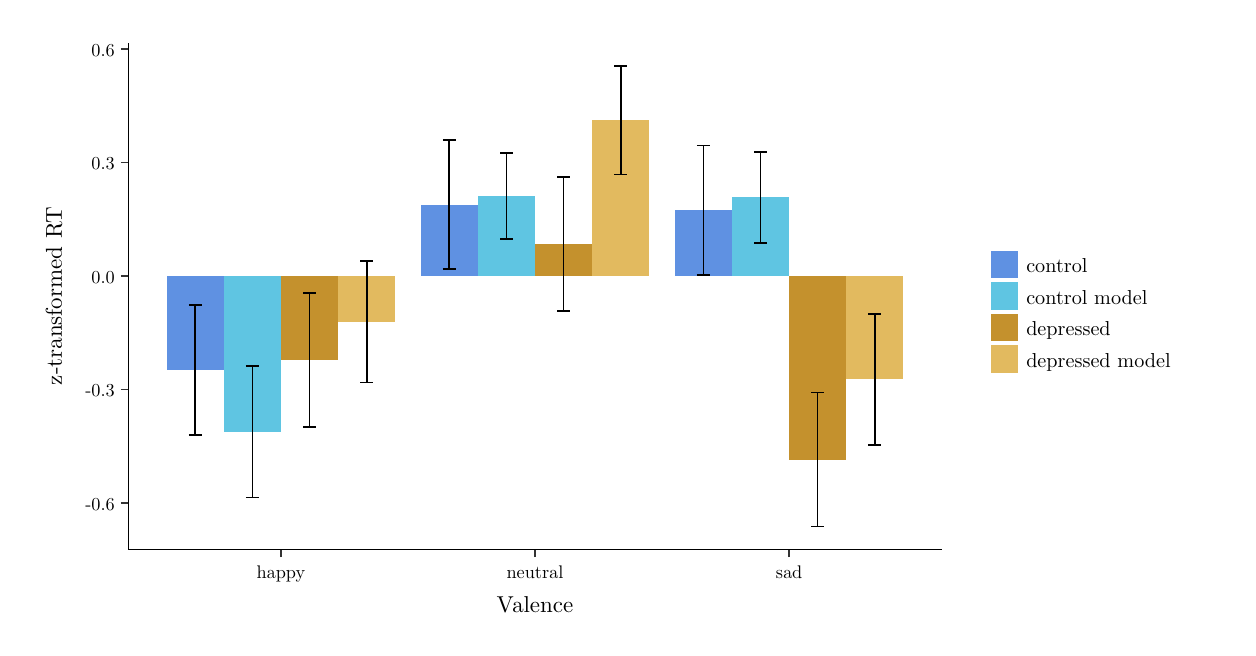
\begin{tikzpicture}[x=1pt,y=1pt]
\definecolor{fillColor}{RGB}{255,255,255}
\path[use as bounding box,fill=fillColor,fill opacity=0.00] (0,0) rectangle (433.62,216.81);
\begin{scope}
\path[clip] (  0.00,  0.00) rectangle (433.62,216.81);
\definecolor{drawColor}{RGB}{255,255,255}
\definecolor{fillColor}{RGB}{255,255,255}

\path[draw=drawColor,line width= 0.6pt,line join=round,line cap=round,fill=fillColor] (  0.00,  0.00) rectangle (433.62,216.81);
\end{scope}
\begin{scope}
\path[clip] ( 36.43, 28.22) rectangle (330.22,211.31);
\definecolor{fillColor}{RGB}{255,255,255}

\path[fill=fillColor] ( 36.43, 28.22) rectangle (330.22,211.31);
\definecolor{fillColor}{RGB}{226,186,95}

\path[fill=fillColor] (112.17,110.52) rectangle (132.83,127.12);
\definecolor{fillColor}{RGB}{196,145,45}

\path[fill=fillColor] ( 91.51, 96.72) rectangle (112.17,127.12);
\definecolor{fillColor}{RGB}{95,197,226}

\path[fill=fillColor] ( 70.85, 70.83) rectangle ( 91.51,127.12);
\definecolor{fillColor}{RGB}{95,145,226}

\path[fill=fillColor] ( 50.20, 93.15) rectangle ( 70.85,127.12);
\definecolor{fillColor}{RGB}{226,186,95}

\path[fill=fillColor] (203.98,127.12) rectangle (224.64,183.35);
\definecolor{fillColor}{RGB}{196,145,45}

\path[fill=fillColor] (183.32,127.12) rectangle (203.98,138.59);
\definecolor{fillColor}{RGB}{95,197,226}

\path[fill=fillColor] (162.66,127.12) rectangle (183.32,156.00);
\definecolor{fillColor}{RGB}{95,145,226}

\path[fill=fillColor] (142.01,127.12) rectangle (162.66,152.86);
\definecolor{fillColor}{RGB}{226,186,95}

\path[fill=fillColor] (295.79, 89.73) rectangle (316.45,127.12);
\definecolor{fillColor}{RGB}{196,145,45}

\path[fill=fillColor] (275.13, 60.74) rectangle (295.79,127.12);
\definecolor{fillColor}{RGB}{95,197,226}

\path[fill=fillColor] (254.47,127.12) rectangle (275.13,155.52);
\definecolor{fillColor}{RGB}{95,145,226}

\path[fill=fillColor] (233.82,127.12) rectangle (254.47,150.85);
\definecolor{drawColor}{RGB}{0,0,0}

\path[draw=drawColor,line width= 0.6pt,line join=round] (120.20,132.43) --
	(124.79,132.43);

\path[draw=drawColor,line width= 0.6pt,line join=round] (122.50,132.43) --
	(122.50, 88.60);

\path[draw=drawColor,line width= 0.6pt,line join=round] (120.20, 88.60) --
	(124.79, 88.60);

\path[draw=drawColor,line width= 0.6pt,line join=round] ( 99.54,120.91) --
	(104.14,120.91);

\path[draw=drawColor,line width= 0.6pt,line join=round] (101.84,120.91) --
	(101.84, 72.52);

\path[draw=drawColor,line width= 0.6pt,line join=round] ( 99.54, 72.52) --
	(104.14, 72.52);

\path[draw=drawColor,line width= 0.6pt,line join=round] ( 78.89, 94.61) --
	( 83.48, 94.61);

\path[draw=drawColor,line width= 0.6pt,line join=round] ( 81.18, 94.61) --
	( 81.18, 47.05);

\path[draw=drawColor,line width= 0.6pt,line join=round] ( 78.89, 47.05) --
	( 83.48, 47.05);

\path[draw=drawColor,line width= 0.6pt,line join=round] ( 58.23,116.57) --
	( 62.82,116.57);

\path[draw=drawColor,line width= 0.6pt,line join=round] ( 60.53,116.57) --
	( 60.53, 69.74);

\path[draw=drawColor,line width= 0.6pt,line join=round] ( 58.23, 69.74) --
	( 62.82, 69.74);

\path[draw=drawColor,line width= 0.6pt,line join=round] (212.01,202.99) --
	(216.60,202.99);

\path[draw=drawColor,line width= 0.6pt,line join=round] (214.31,202.99) --
	(214.31,163.71);

\path[draw=drawColor,line width= 0.6pt,line join=round] (212.01,163.71) --
	(216.60,163.71);

\path[draw=drawColor,line width= 0.6pt,line join=round] (191.35,162.86) --
	(195.95,162.86);

\path[draw=drawColor,line width= 0.6pt,line join=round] (193.65,162.86) --
	(193.65,114.33);

\path[draw=drawColor,line width= 0.6pt,line join=round] (191.35,114.33) --
	(195.95,114.33);

\path[draw=drawColor,line width= 0.6pt,line join=round] (170.70,171.57) --
	(175.29,171.57);

\path[draw=drawColor,line width= 0.6pt,line join=round] (172.99,171.57) --
	(172.99,140.43);

\path[draw=drawColor,line width= 0.6pt,line join=round] (170.70,140.43) --
	(175.29,140.43);

\path[draw=drawColor,line width= 0.6pt,line join=round] (150.04,176.20) --
	(154.63,176.20);

\path[draw=drawColor,line width= 0.6pt,line join=round] (152.34,176.20) --
	(152.34,129.53);

\path[draw=drawColor,line width= 0.6pt,line join=round] (150.04,129.53) --
	(154.63,129.53);

\path[draw=drawColor,line width= 0.6pt,line join=round] (303.82,113.43) --
	(308.41,113.43);

\path[draw=drawColor,line width= 0.6pt,line join=round] (306.12,113.43) --
	(306.12, 66.03);

\path[draw=drawColor,line width= 0.6pt,line join=round] (303.82, 66.03) --
	(308.41, 66.03);

\path[draw=drawColor,line width= 0.6pt,line join=round] (283.16, 84.93) --
	(287.75, 84.93);

\path[draw=drawColor,line width= 0.6pt,line join=round] (285.46, 84.93) --
	(285.46, 36.55);

\path[draw=drawColor,line width= 0.6pt,line join=round] (283.16, 36.55) --
	(287.75, 36.55);

\path[draw=drawColor,line width= 0.6pt,line join=round] (262.51,171.96) --
	(267.10,171.96);

\path[draw=drawColor,line width= 0.6pt,line join=round] (264.80,171.96) --
	(264.80,139.08);

\path[draw=drawColor,line width= 0.6pt,line join=round] (262.51,139.08) --
	(267.10,139.08);

\path[draw=drawColor,line width= 0.6pt,line join=round] (241.85,174.18) --
	(246.44,174.18);

\path[draw=drawColor,line width= 0.6pt,line join=round] (244.15,174.18) --
	(244.15,127.51);

\path[draw=drawColor,line width= 0.6pt,line join=round] (241.85,127.51) --
	(246.44,127.51);
\end{scope}
\begin{scope}
\path[clip] (  0.00,  0.00) rectangle (433.62,216.81);
\definecolor{drawColor}{RGB}{0,0,0}

\path[draw=drawColor,line width= 0.6pt,line join=round] ( 36.43, 28.22) --
	( 36.43,211.31);
\end{scope}
\begin{scope}
\path[clip] (  0.00,  0.00) rectangle (433.62,216.81);
\definecolor{drawColor}{RGB}{0,0,0}

\node[text=drawColor,anchor=base east,inner sep=0pt, outer sep=0pt, scale=  0.66] at ( 31.48, 42.38) {-0.6};

\node[text=drawColor,anchor=base east,inner sep=0pt, outer sep=0pt, scale=  0.66] at ( 31.48, 83.38) {-0.3};

\node[text=drawColor,anchor=base east,inner sep=0pt, outer sep=0pt, scale=  0.66] at ( 31.48,124.39) {0.0};

\node[text=drawColor,anchor=base east,inner sep=0pt, outer sep=0pt, scale=  0.66] at ( 31.48,165.40) {0.3};

\node[text=drawColor,anchor=base east,inner sep=0pt, outer sep=0pt, scale=  0.66] at ( 31.48,206.40) {0.6};
\end{scope}
\begin{scope}
\path[clip] (  0.00,  0.00) rectangle (433.62,216.81);
\definecolor{drawColor}{gray}{0.20}

\path[draw=drawColor,line width= 0.6pt,line join=round] ( 33.68, 45.10) --
	( 36.43, 45.10);

\path[draw=drawColor,line width= 0.6pt,line join=round] ( 33.68, 86.11) --
	( 36.43, 86.11);

\path[draw=drawColor,line width= 0.6pt,line join=round] ( 33.68,127.12) --
	( 36.43,127.12);

\path[draw=drawColor,line width= 0.6pt,line join=round] ( 33.68,168.12) --
	( 36.43,168.12);

\path[draw=drawColor,line width= 0.6pt,line join=round] ( 33.68,209.13) --
	( 36.43,209.13);
\end{scope}
\begin{scope}
\path[clip] (  0.00,  0.00) rectangle (433.62,216.81);
\definecolor{drawColor}{RGB}{0,0,0}

\path[draw=drawColor,line width= 0.6pt,line join=round] ( 36.43, 28.22) --
	(330.22, 28.22);
\end{scope}
\begin{scope}
\path[clip] (  0.00,  0.00) rectangle (433.62,216.81);
\definecolor{drawColor}{gray}{0.20}

\path[draw=drawColor,line width= 0.6pt,line join=round] ( 91.51, 25.47) --
	( 91.51, 28.22);

\path[draw=drawColor,line width= 0.6pt,line join=round] (183.32, 25.47) --
	(183.32, 28.22);

\path[draw=drawColor,line width= 0.6pt,line join=round] (275.13, 25.47) --
	(275.13, 28.22);
\end{scope}
\begin{scope}
\path[clip] (  0.00,  0.00) rectangle (433.62,216.81);
\definecolor{drawColor}{RGB}{0,0,0}

\node[text=drawColor,anchor=base,inner sep=0pt, outer sep=0pt, scale=  0.66] at ( 91.51, 17.82) {happy};

\node[text=drawColor,anchor=base,inner sep=0pt, outer sep=0pt, scale=  0.66] at (183.32, 17.82) {neutral};

\node[text=drawColor,anchor=base,inner sep=0pt, outer sep=0pt, scale=  0.66] at (275.13, 17.82) {sad};
\end{scope}
\begin{scope}
\path[clip] (  0.00,  0.00) rectangle (433.62,216.81);
\definecolor{drawColor}{RGB}{0,0,0}

\node[text=drawColor,anchor=base,inner sep=0pt, outer sep=0pt, scale=  0.83] at (183.32,  5.50) {Valence};
\end{scope}
\begin{scope}
\path[clip] (  0.00,  0.00) rectangle (433.62,216.81);
\definecolor{drawColor}{RGB}{0,0,0}

\node[text=drawColor,rotate= 90.00,anchor=base,inner sep=0pt, outer sep=0pt, scale=  0.83] at ( 12.32,119.77) {z-transformed RT};
\end{scope}
\begin{scope}
\path[clip] (  0.00,  0.00) rectangle (433.62,216.81);
\definecolor{fillColor}{RGB}{255,255,255}

\path[fill=fillColor] (341.60, 85.74) rectangle (428.12,153.80);
\end{scope}
\begin{scope}
\path[clip] (  0.00,  0.00) rectangle (433.62,216.81);
\definecolor{fillColor}{RGB}{95,145,226}

\path[fill=fillColor] (348.00,126.28) rectangle (357.96,136.24);
\end{scope}
\begin{scope}
\path[clip] (  0.00,  0.00) rectangle (433.62,216.81);
\definecolor{fillColor}{RGB}{95,197,226}

\path[fill=fillColor] (348.00,114.90) rectangle (357.96,124.86);
\end{scope}
\begin{scope}
\path[clip] (  0.00,  0.00) rectangle (433.62,216.81);
\definecolor{fillColor}{RGB}{196,145,45}

\path[fill=fillColor] (348.00,103.52) rectangle (357.96,113.48);
\end{scope}
\begin{scope}
\path[clip] (  0.00,  0.00) rectangle (433.62,216.81);
\definecolor{fillColor}{RGB}{226,186,95}

\path[fill=fillColor] (348.00, 92.14) rectangle (357.96,102.10);
\end{scope}
\begin{scope}
\path[clip] (  0.00,  0.00) rectangle (433.62,216.81);
\definecolor{drawColor}{RGB}{0,0,0}

\node[text=drawColor,anchor=base west,inner sep=0pt, outer sep=0pt, scale=  0.73] at (360.84,128.23) {control};
\end{scope}
\begin{scope}
\path[clip] (  0.00,  0.00) rectangle (433.62,216.81);
\definecolor{drawColor}{RGB}{0,0,0}

\node[text=drawColor,anchor=base west,inner sep=0pt, outer sep=0pt, scale=  0.73] at (360.84,116.85) {control model};
\end{scope}
\begin{scope}
\path[clip] (  0.00,  0.00) rectangle (433.62,216.81);
\definecolor{drawColor}{RGB}{0,0,0}

\node[text=drawColor,anchor=base west,inner sep=0pt, outer sep=0pt, scale=  0.73] at (360.84,105.47) {depressed};
\end{scope}
\begin{scope}
\path[clip] (  0.00,  0.00) rectangle (433.62,216.81);
\definecolor{drawColor}{RGB}{0,0,0}

\node[text=drawColor,anchor=base west,inner sep=0pt, outer sep=0pt, scale=  0.73] at (360.84, 94.09) {depressed model};
\end{scope}
\end{tikzpicture}
